\documentclass{article}
\usepackage{graphicx} 
\usepackage{wrapfig} 
%\usepackage[T1]{fontenc}
%\usepackage[polish]{babel}
\usepackage{polski}
\usepackage[utf8]{inputenc}
%\usepackage[latin2]{inputenc}
%\usepackage[polish]{babel}
\usepackage{hyperref}
\begin{document}
Autor: Pawel Lipkowski\newline
\newline
\section{Co to jest figura obrotowa?}
	\subsection{Definicja}
		 Figura obrotowa jest to bryła geometryczna ograniczona powierzchnią powstałą z obrotu figury plaskiej dookoła prostej (osi obrotu).~\cite{def}
	\subsection{Przykłady figur obrotowych}
		\begin{itemize}
 			\item walec
 			\item stożek (konus, pachołek)
 			\item kula
			\item figury powstałe w wyniku obrotu wykresow funkcji
			\item elipsoida obrotowa
			\item torus (innymi słowy paczek, obwarzanek, dętka etc)
			\item beczka
			\begin{enumerate}
  				\item hiperboloida obrotowa
  				\item paraboloida obrotowa etc \ldots
			\end{enumerate}
		\end{itemize}
		%\begin{figure}
		%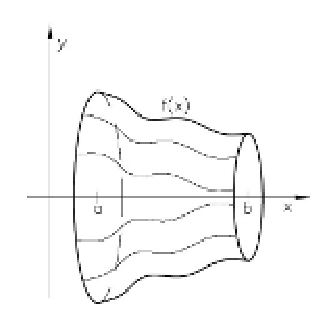
\includegraphics{k.eps}
		%\end{figure}
		%\newpage
\section{Pola i objętości figur obrotowych}
	\subsection{Wzory ogólne}
		\subsection{Objętość}
			$V = \pi \int_{a}^{b}(f(x))^{2}dx $	
		\subsection{Pole powierzchni (parametrycznie)}
			$V = 2 \pi \int_{t1}^{t2} |y(t)| \sqrt{[x'(t)]^2 + [y'(t)]^2} dt $
	\subsection{Wzory dla konkretnych figur}	
	\begin{tabular}{|c|c|c|}
 	\hline 
 	Figura & Pole & Objjętość \\
 	\hline
 	Walec & $2\pi r^{2} + 2\pi rh$ & $\pi r^{2}h$  \\
	\hline
 	Stozek & $\pi r^{2} + \pi rl$ & $\frac{1}{3}\pi r^{2}h$  \\
  	\hline
  	Kula & $4\pi r^{2}$ & $\frac{4}{3}\pi r^{3}$  \\
  	\hline
	\end{tabular} 
	\begin{thebibliography}{99}
	\bibitem{def} \url{https://pl.wikipedia.org/wiki/Bry%C5%82a_obrotowa}
	\end{thebibliography}
	
	\begin{wrapfigure}{r}{0.5\textwidth}
	%\begin{center}
	\vspace{-20pt}
	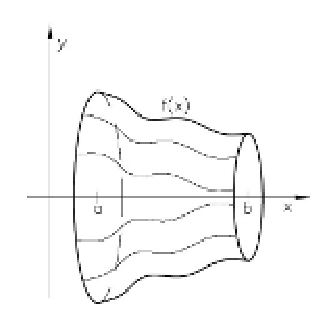
\includegraphics[width=0.48\textwidth]{k}
	%\end{center}
	\vspace{-20pt}
	\caption{Bryła obrotowa powstała w wyniku obrotu figury ograniczonej funkcją f(x) z przedziału od a do b}
	\vspace{-10pt}
	\end{wrapfigure}
\end{document}
